\documentclass[a4paper, 12pt]{article}
\usepackage[utf8]{inputenc}
\usepackage[T1]{fontenc}
\usepackage[french]{babel}
\usepackage{eurosym}
\usepackage{graphicx}
\usepackage{listings}
\usepackage{color}
\usepackage{caption}
\usepackage{courier}
\usepackage{eso-pic,xcolor,graphicx}

\setcounter{tocdepth}{3}
\setcounter{secnumdepth}{3}


%PAGE DE COUVERTURE -> A revoir , en générer une bien stylé
\makeatletter
\def\maketitle{
  \null
  \thispagestyle{empty}
  \vfill
  \begin{center}\leavevmode
    \normalfont
    {\LARGE \@title\par}
    \vskip 1cm
    {\Large \@author\par}
    \vskip 1cm
    {\Large \@date\par}
  \end{center}
  \vfill
  \null
  \cleardoublepage
  }
\makeatother
\title{PROJET MACSI1 : Réalisation d'une application de gestion de projet }
\author{RUCKEBUSCH Arnaud - NORBAL Xavier - JOULOT Philippe - NAHA Myriam}
\date{Encadrant : Yeha Taher}


%%% PARAMETRES INSERTION DE CODE %%%%%%
\lstset{
         basicstyle=\footnotesize\ttfamily,
        % numbers=left,             
         numberstyle=\tiny,          
        % stepnumber=2,            
         numbersep=5pt,             
         tabsize=2,                 
         extendedchars=true,         
         breaklines=true,           
         keywordstyle=\color{red},
    		frame=b,         
 %        keywordstyle=[1]\textbf,    % Stil der Keywords
 %        keywordstyle=[2]\textbf,    %
 %        keywordstyle=[3]\textbf,    %
 %        keywordstyle=[4]\textbf,   \sqrt{\sqrt{}} %
         stringstyle=\color{white}\ttfamily, 
         showspaces=false,           
         showtabs=false,             
         xleftmargin=17pt,
         framexleftmargin=17pt,
         framexrightmargin=5pt,
         framexbottommargin=4pt,
	frame = single;
	breakatwhitespace=true,
         %backgroundcolor=\color{lightgray},
        % showstringspaces=false      
	title=\lstname 
 }
 \lstloadlanguages{% Check Dokumentation for further languages ...
         %[Visual]Basic
         %Pascal
         %C
         %C++
         XML,
         %HTML
         Java,
         SQL
 }


  %\captionsetup[lstlisting]{singlelinecheck=false, labelfont={blue}, textfont={blue}}





%DEBUT DU DOCUMENT

\begin{document}

\begin{figure}[h!]
	
\includegraphics[width=1\textwidth]{GESPRO2014.png}
\end{figure}
\maketitle

\setcounter{page}{1}
\tableofcontents
\newpage



\section{Introduction}
\paragraph{}La bonne gestion de projet est un problème récurent, ce projet a pour but de nous apprendre un processus de gestion de projet étant très grandement utilisé dans différent domaines et plus particulièrement en informatique. Le but final est de réaliser une application permettant la gestion de projet suivant le processus décrit.

\newpage

\section{Approche du sujet et conception du modèle}

\subsection{Les outils utilisés}
\paragraph{}Pour ce projet et pour nous simplifier le travail de groupe nous avons utilisés GIT (outils de gestion de version très répandu), notepad++ pour effectuer toute la partie rédaction du code, easyphp/wamp afin de tester notre application en mode local, starUML pour la réalisation du diagramme de classe, ainsi que TexWorks pour la rédaction de ce rapport..

\subsection{Modèle de classe}

\begin{figure}[h!]
	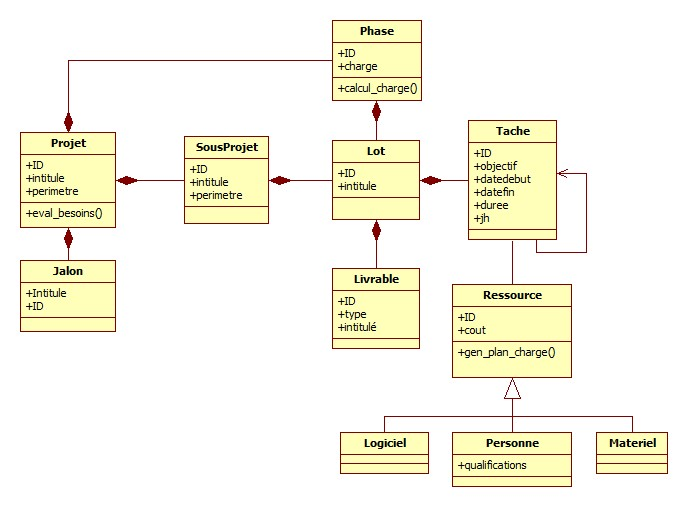
\includegraphics[height=4cm]{diagramme_de_classe.jpg}
	\caption{Diagramme de classe}
\end{figure}
\paragraph{}Pour ce diagramme de classe nous avons choisis de ne pas créer de classe tableau de bord, car nous pensons que cela correspond plus à une méthode qui va générer ce tableau de bord en fonction des autres informations du diagramme.
\paragraph{}Un projet est composé de sous projets qui sont eux mêmes composés de lots qui sont eux mêmes composés de phases. Un projet est également composé de phases qui est associé à 1 ou plusieurs livrables qui sont généré par les jalons. Les taches dépendent d'elles mêmes et ont chacune un taux d'affectation de ressources qui peuvent être de types humains, logistiques ou bien physiques.

\newpage

\section{Transformation du modèle}
\subsection{Méthode de transformation}
\paragraph{}Pour transformer le diagramme de classe précédent en modèle relationnel nous avons simplement appliqué les principes du cours de macsi1 en commençant par les spécialisations, s'en suit les relations et nous finissons par les agrégations pour arriver au modèle relationnel ci dessous.
\subsection{Modèle relationnel}
\paragraph{} // Photo du 3FN final
\paragraph{} //Ajout descriptions pour chaque éléments et pk on a descnedus certains éléments
\subsection{Eléments 3FN et cohérence}
\paragraph{} //Passage en  3FN

\newpage

\section{Conception}
\subsection{Implémentation de la base de données}
\paragraph{}Le modèle 3FN n'est pas toujours le plus efficace, en effet suivant les jointures que nous faisons régulièrement ou bien les restrictions courantes il peut-être utile de démoraliser afin d'obtenir des tables plus grandes mais permettant une meilleure intégrité des données et ceci sans perte d'information. Nous avons donc choisis la BD suivante :
\\ \\
\lstinputlisting[language=SQL]{BD_MACSI1.sql}
\newpage
\subsection{Dévéloppement de l'application}
\paragraph{}Comme énoncé précemment nous avons utilisés plusieurs outils pour le développement de notre application. Nous avons également fait le choix de développer cette application en html-css-php principalement car nous préférons ce langage à d'autres et que la gestion de la base de données s'y préttait bien. Nous avons également utilisé du javascript notamment pour afficher des calendrier lors de la sélection de dates, ainsi que de l'ajax pour avoir des formulaires dynamiques.
\paragraph{}Nous nous sommes répartis les différentes parties du projet afin de pouvoir les implémenter de manière parallèlles et ainsi profiter au mieux de notre système de gestion de version sans créer trop de conflit lors de nos différents push.

\newpage
\subsection{Difficultées recontrées}
\paragraph{}Lors de ce projet les principales difficultés furent l'élaboration du modèle ainsi que la base de donnée, étant des élément clés pour tout le développement du projet il fallait bien être sur qu'avant de coder ces modèles étaient correct et que nous n'aurions pas à revenir dessus au cours du projet, sans quoi de nombreuses choses auraient été à modifier. Maitrisant bien le langage web et il été plus long que difficile d'implémenter notre plateforme.




\newpage

\section{Présentation de l'application}


\newpage

\section{Bibliographie}
\subsection{Logiciels}
\begin{enumerate}
	\item Git
	\item Photophiltre
	\item EasyPHP / wamp
	\item TeXworks
	\item Notepad++
\end{enumerate}

\subsection{Recherche d’informations}
\begin{enumerate}
	\item Github.com
	\item Easyphp.com
	\item Php.net
	\item Cours de macsi1 du premier semestre
	\item Wikibooks section LaTex
\end{enumerate}

\newpage

\section{Conclusion}
\paragraph{}Pour conclure, ce projet nous a permis de bien aborder ce processus de gestion de projet en le concrétisant dans la réalisation d'une application. Les différentes étapes du projet nous ont également permis de mettre a profit nos connaissances dans la conception, transformation de modèle et création de base de données ainsi que dans les langages web HTML/CSS/PHP/MYSQL que nous avons utilisés pour la réalisation de l'application.

\end{document}





















